% (find-LATEX "2020-1-C2-P1.tex")
% (defun c () (interactive) (find-LATEXsh "lualatex -record 2020-1-C2-P1.tex" :end))
% (defun D () (interactive) (find-pdf-page      "~/LATEX/2020-1-C2-P1.pdf"))
% (defun d () (interactive) (find-pdftools-page "~/LATEX/2020-1-C2-P1.pdf"))
% (defun e () (interactive) (find-LATEX "2020-1-C2-P1.tex"))
% (defun u () (interactive) (find-latex-upload-links "2020-1-C2-P1"))
% (defun v () (interactive) (find-2a '(e) '(d)) (g))
% (find-pdf-page   "~/LATEX/2020-1-C2-P1.pdf")
% (find-sh0 "cp -v  ~/LATEX/2020-1-C2-P1.pdf /tmp/")
% (find-sh0 "cp -v  ~/LATEX/2020-1-C2-P1.pdf /tmp/pen/")
%   file:///home/edrx/LATEX/2020-1-C2-P1.pdf
%               file:///tmp/2020-1-C2-P1.pdf
%           file:///tmp/pen/2020-1-C2-P1.pdf
% http://angg.twu.net/LATEX/2020-1-C2-P1.pdf
% (find-LATEX "2019.mk")
% (find-C2-aula-links "2020-1-C2-P1" "p1" "p1")

% «.defs»			(to "defs")
% «.title»			(to "title")
% «.regras»			(to "regras")
% «.questao-1»			(to "questao-1")
% «.questao-2»			(to "questao-2")
% «.questao-3»			(to "questao-3")
% «.questao-4»			(to "questao-4")
% «.gabarito-2a»		(to "gabarito-2a")
% «.gabarito-2b»		(to "gabarito-2b")
% «.gabarito-3a»		(to "gabarito-3a")
% «.scans»			(to "scans")
% «.comentario-telegram»	(to "comentario-telegram")

\documentclass[oneside,12pt]{article}
\usepackage[colorlinks,citecolor=DarkRed,urlcolor=DarkRed]{hyperref} % (find-es "tex" "hyperref")
\usepackage{amsmath}
\usepackage{amsfonts}
\usepackage{amssymb}
\usepackage{pict2e}
\usepackage[x11names,svgnames]{xcolor} % (find-es "tex" "xcolor")
%\usepackage{colorweb}                 % (find-es "tex" "colorweb")
%\usepackage{tikz}
%
% (find-dn6 "preamble6.lua" "preamble0")
%\usepackage{proof}   % For derivation trees ("%:" lines)
%\input diagxy        % For 2D diagrams ("%D" lines)
%\xyoption{curve}     % For the ".curve=" feature in 2D diagrams
%
\usepackage{edrx15}               % (find-LATEX "edrx15.sty")
\input edrxaccents.tex            % (find-LATEX "edrxaccents.tex")
\input edrxchars.tex              % (find-LATEX "edrxchars.tex")
\input edrxheadfoot.tex           % (find-LATEX "edrxheadfoot.tex")
\input edrxgac2.tex               % (find-LATEX "edrxgac2.tex")
%
%\usepackage[backend=biber,
%   style=alphabetic]{biblatex}            % (find-es "tex" "biber")
%\addbibresource{catsem-slides.bib}        % (find-LATEX "catsem-slides.bib")
%
% (find-es "tex" "geometry")
\usepackage[a6paper, landscape,
            top=1.5cm, bottom=.25cm, left=1cm, right=1cm, includefoot
           ]{geometry}
%
\begin{document}

\catcode`\^^J=10
\directlua{dofile "dednat6load.lua"}  % (find-LATEX "dednat6load.lua")

% %L dofile "edrxtikz.lua"  -- (find-LATEX "edrxtikz.lua")
% %L dofile "edrxpict.lua"  -- (find-LATEX "edrxpict.lua")
% \pu

% «defs»  (to ".defs")
% (find-LATEX "edrx15.sty" "colors-2019")
\long\def\ColorRed   #1{{\color{Red1}#1}}
\long\def\ColorViolet#1{{\color{MagentaVioletLight}#1}}
\long\def\ColorViolet#1{{\color{Violet!50!black}#1}}
\long\def\ColorGreen #1{{\color{SpringDarkHard}#1}}
\long\def\ColorGreen #1{{\color{SpringGreenDark}#1}}
\long\def\ColorGreen #1{{\color{SpringGreen4}#1}}
\long\def\ColorGray  #1{{\color{GrayLight}#1}}
\long\def\ColorGray  #1{{\color{black!30!white}#1}}
\long\def\ColorBrown #1{{\color{Brown}#1}}
\long\def\ColorBrown #1{{\color{brown}#1}}

\long\def\ColorShort #1{{\color{SpringGreen4}#1}}
\long\def\ColorLong  #1{{\color{Red1}#1}}

\def\frown{\ensuremath{{=}{(}}}
\def\True {\mathbf{V}}
\def\False{\mathbf{F}}
\def\D    {\displaystyle}
\def\S{\sen x}
\def\C{\cos x}

\def\drafturl{http://angg.twu.net/LATEX/2020-1-C2.pdf}
\def\drafturl{http://angg.twu.net/2020.1-C2.html}
\def\draftfooter{\tiny \href{\drafturl}{\jobname{}} \ColorBrown{\shorttoday{} \hours}}

% (find-angg ".emacs" "c2q192")


%  _____ _ _   _                               
% |_   _(_) |_| | ___   _ __   __ _  __ _  ___ 
%   | | | | __| |/ _ \ | '_ \ / _` |/ _` |/ _ \
%   | | | | |_| |  __/ | |_) | (_| | (_| |  __/
%   |_| |_|\__|_|\___| | .__/ \__,_|\__, |\___|
%                      |_|          |___/      
%
% «title»  (to ".title")
% (c2m201p1p 1 "title")
% (c2m201p1a   "title")

\thispagestyle{empty}

\begin{center}

\vspace*{1.2cm}

{\bf \Large Cálculo 2 - 2020.1}

\bsk

P1 (Primeira prova)

\bsk

Eduardo Ochs - RCN/PURO/UFF

\url{http://angg.twu.net/2020.1-C2.html}

\end{center}

\newpage

% «regras»  (to ".regras")
% (c2m201p1p 2 "regras")
% (c2m201p1a   "regras")
% (c2m201mt1p 7 "miniteste-regras")
% (c2m201mt1    "miniteste-regras")
% (c3m201pltanp 11 "mini-teste-1")
% (c3m201pltan     "mini-teste-1")

{\bf Regras para a P1:}

\ssk

As questões da P1 serão disponibilizadas às 16:00 da
quinta-feira 19/nov/2020 e você deverá entregar as respostas
\ColorRed{escritas à mão} até as 16:00 da sexta-feira 20/nov/2020 na
plataforma Classroom. Se o Classroom der algum problema mande também
para este endereço de e-mail:

\ssk

\ColorRed{eduardoochs@gmail.com}

\ssk

Provas entregues após este horário não serão considerados.

Durante as 24 horas do mini-teste nem o professor nem o monitor
responderão perguntas sobre os assuntos do mini-teste, mas você pode
discutir com os seus colegas e até com as pessoas do grupo da outra
turma... \ColorRed{só que as respostas devem ser individuais}.

% {\bf Regras (cont.):}
% 
% \ssk
% 
% Os alunos que cumprirem uma série de condições (ainda não divulguei a
% lista delas...) poderão compensar as suas questões erradas na P2
% fazendo vídeos explicando passo a passo como resolvê-las na semana
% seguinte à prova. \ColorRed{Uma das condições é ter feito todos os
%   mini-testes, então não deixe de fazer e entregar este mini-teste!}

\newpage

% «questao-1»  (to ".questao-1")
% (c2m201p1p 3 "questao-1")
% (c2m201p1a   "questao-1")
% (find-es "ipython" "2020.1-C2-P1")

{\bf Questão 1}

(Total: 2.5 pts)

\ssk

Seja $f(x) = x^2 - 1$.

Seja [Trap] o somatório que corresponde ao método do trapézio.

a) (0.3 pts) Represente graficamente $\Intx{0}{2}{f(x)}$.

b) (0.3 pts) Represente graficamente [Trap]

   para a partição $P=\{0,1,2\}$.

c) (0.3 pts) Represente graficamente [Trap]

   para a partição $P=\{0,2\}$.

d) (1.0 pts) Calcule $\Intx{0}{2}{f(x)}$.

e) (0.3 pts) Calcule [Trap] para $P=\{0,1,2\}$.

f) (0.3 pts) Calcule [Trap] para $P=\{0,2\}$.


\newpage

% «questao-2»  (to ".questao-2")
% (c2m201p1p 4 "questao-2")
% (c2m201p1a   "questao-2")

{\bf Questão 2}

(Total: 2.5 pts)

\ssk

a) (1.5 pts) Calcule $\D \intx{\ln(2x+3)}$.

b) (1.0 pts) Teste a sua resposta.

\bsk

Dica: aqui você vai precisar usar integração por partes e integração
por substituição. Esta questão é um pouco mais difícil do que as
integrações por partes que nós vimos nas aulas, consulte os livros pra
ter idéias de como fazê-la.

\newpage

% «questao-3»  (to ".questao-3")
% (c2m201p1p 5 "questao-3")
% (c2m201p1a   "questao-3")

{\bf Questão 3}

(Total: 2.5 pts)

\ssk

a) (1.5 pts) Calcule $\D \intx{\frac{x^3}{x^2 + 5x + 6}}$.

b) (1.0 pts) Teste a sua resposta.

\newpage

% «questao-4»  (to ".questao-4")
% (c2m201p1p 6 "questao-4")
% (c2m201p1a   "questao-4")

{\bf Questão 4}

(Total: 2.5 pts)

\ssk

a) (1.0 pts) Calcule $\D \intx{(\S)^5 (\C)^3}$

\ColorRed{usando a substituição $c=\cos x$}.

\ssk

b) (1.5 pts) Teste a sua resposta.


\newpage

% «gabarito-2a»  (to ".gabarito-2a")
% (c2m201p1p 7 "gabarito-2a")
% (c2m201p1a   "gabarito-2a")
% (find-latexscan-links "C2" "20201201_p1gab_2a")
% (find-xpdf-page "~/LATEX/2020-1-C2/20201201_p1gab_2a.pdf")
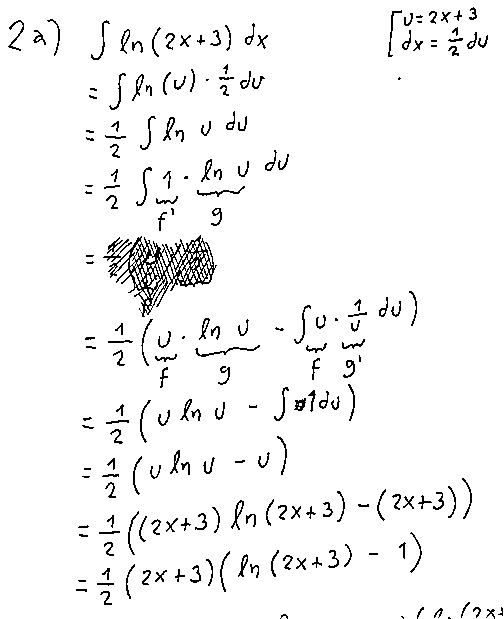
\includegraphics[height=8cm]{2020-1-C2/20201201_p1gab_2a.pdf}
%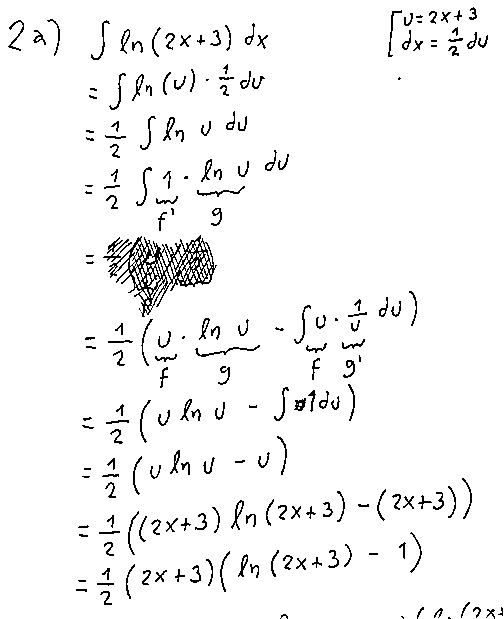
\includegraphics[width=11cm]{2020-1-C2/20201201_p1gab_2a.pdf}

\newpage

% «gabarito-2b»  (to ".gabarito-2b")
% (c2m201p1p 8 "gabarito-2b")
% (c2m201p1a   "gabarito-2b")
% (find-latexscan-links "C2" "20201201_p1gab_2b")
% (find-xpdf-page "~/LATEX/2020-1-C2/20201201_p1gab_2b.pdf")
%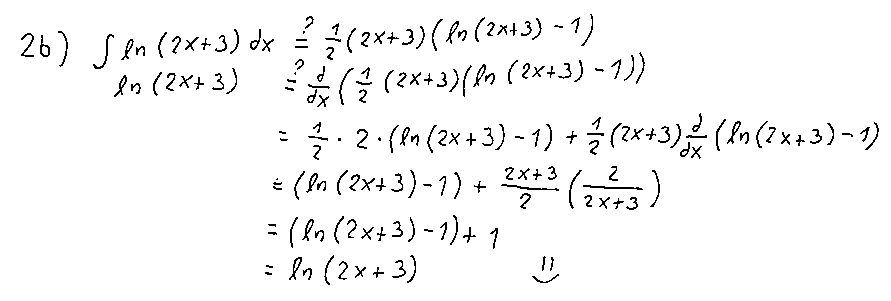
\includegraphics[height=8cm]{2020-1-C2/20201201_p1gab_2b.pdf}
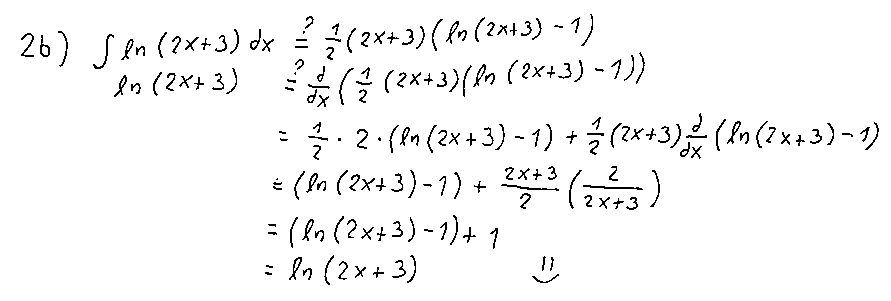
\includegraphics[width=11cm]{2020-1-C2/20201201_p1gab_2b.pdf}

\newpage

% «gabarito-3a»  (to ".gabarito-3a")
% (c2m201p1p 9 "gabarito-3a")
% (c2m201p1a   "gabarito-3a")
% (find-latexscan-links "C2" "20201201_p1gab_3a")
% (find-xpdf-page "~/LATEX/2020-1-C2/20201201_p1gab_3a.pdf")

\includegraphics[height=8cm]{2020-1-C2/20201201_p1gab_3a.pdf}
%
\includegraphics[width=11cm]{2020-1-C2/20201201_p1gab_3a.pdf}


\newpage

% «comentario-telegram»  (to ".comentario-telegram")
% (c2m201p1p 10 "comentario-telegram")
% (c2m201p1a    "comentario-telegram")

{\bf Comentário sobre a P1 (no grupo do Telegram)}

\ssk

Oi! Vou voltar às correções agora e espero terminar todas as P1s daqui
a pouco.

Algumas pessoas que tiraram notas baixas me perguntaram em privado o
que elas erraram na prova. Vou responder por aqui porque acho que a
resposta é útil pra todo mundo e vale pra P2 também.

Era uma prova pra ser feita em 24 horas, com consulta e com discussão
com os colegas, então os critérios de correção são bem diferentes dos
critérios pra uma prova individual de duas horas... vou usar como
exemplo frações parciais.

Eu esperava que quando vocês tivessem terminado a prova vocês
soubessem frações parciais muito bem e lembrassem como era só saber as
idéias básicas de frações parciais, mas não saber nem fazer as contas
direito... e aí era pra vocês terem resolvido a questão de frações
parciais da prova da forma mais clara possível, no seguinte sentido:
eu esperava que a solução da questão de frações parciais de vocês
fosse como uma explicação bem detalhada de como resolver aquele
problema, {\it como se vocês estivessem ensinando frações parciais pra
  alguém que ainda não entendeu direito}.

Deveria ser fácil entender cada ``='' de vocês, e as partes em que vocês
fazem a divisão com resto e encontram o A e o B do sistema deveriam
estar claramente separadas do resto.

E eu esperava que vocês tivessem relido e revisado várias vezes as
soluções de vocês, e reescrito as partes que não tivessem ficado
claras quando vocês escreveram elas da primeira vez. Eu esperava que
vocês mostrassem que tinham virado as pessoas que sabem frações
parciais bastante bem.

Na questão sobre integrar $(\sen x)^5 (\cos x)^3$ várias pessoas
fizeram uma coisa que me deixou BEM puto. Nas contas essas várias
pessoas escreveram um ``menos'' no lugar que deveria ter um ``vezes''
- todas cometeram o mesmo erro no mesmo lugar. E isso pra mim foi
sinal de que as pessoas não aprenderam o suficiente sobre aquela parte
da matéria pra conseguirem revisar aquelas contas - e que elas achavam
que não precisavam aprender, bastava copiar.




\end{document}

% «scans»  (to ".scans")
% (find-LATEX "2020-1-C3-aprox-2a-ordem-R2.tex" "scans")

 (eepitch-shell)
 (eepitch-kill)
 (eepitch-shell)
# (find-fline "~/2020.1-C2/")
# (find-fline "~/2020.1-C3/")
# (find-fline "~/LATEX/2020-1-C2/")
# (find-fline "~/LATEX/2020-1-C3/")
# (find-fline "/tmp/c2trigsubst1/")
# (find-fline "/tmp/c2gab/")
# (find-fline "/tmp/")
cd /tmp/qc3/
cd /tmp/c2trigsubst1/
cd /tmp/
cd /tmp/c2gab/
for i in *.jpg; do echo f $(basename $i .jpg); done

f () { rm -fv $1.png $1.pdf; djvuize $1.pdf }
f () { rm -fv $1.png $1.pdf; djvuize WHITEBOARDOPTS="-m 0.5" $1.pdf; xpdf $1.pdf }
f () { rm -fv $1.png $1.pdf; djvuize WHITEBOARDOPTS="-m 0.25" $1.pdf; xpdf $1.pdf }
f () { cp -fv $1.png $1.pdf       ~/2020.1-C3/ }
f () { cp -fv        $1.pdf ~/LATEX/2020-1-C3/ }
f () { cp -fv $1.png $1.pdf       ~/2020.1-C2/
       cp -fv        $1.pdf ~/LATEX/2020-1-C2/
       cat <<%%%
% (find-latexscan-links "C2" "$1")
%%%
}

f 20201201_p1gab_2a
f 20201201_p1gab_2b
f 20201201_p1gab_3a

# (find-man "busybox")
# (find-man "basename")


f 20201202_substtrig_grande
f 20201202_substtrig_ids_e_blocos
f 20201202_substtrig_t
f 20201202_substtrig_z

f 20201126_strig_teste

f 20201125_160159_exerc_1
f 20201125_160249_abreviacoes
f 20201125_160341_substituicao_s


%  __  __       _        
% |  \/  | __ _| | _____ 
% | |\/| |/ _` | |/ / _ \
% | |  | | (_| |   <  __/
% |_|  |_|\__,_|_|\_\___|
%                        
% <make>

 (eepitch-shell)
 (eepitch-kill)
 (eepitch-shell)
# (find-LATEXfile "2019planar-has-1.mk")
make -f 2019.mk STEM=2020-1-C2-P1 veryclean
make -f 2019.mk STEM=2020-1-C2-P1 pdf

% Local Variables:
% coding: utf-8-unix
% ee-tla: "c2m201p1"
% End:
